\chapter{Definição do Problema de Escalonamento de Tarefas e Alocação de Dados de WfCs em Nuvem}\label{chap4}


Neste capítulo, o modelo matemático para o problema de escalonamento de tarefas e alocação de arquivos é apresentado. Primeiramente serão discutidos os modelos relacionados à aplicação e ao ambiente de execução. Em seguida, a formulação matemática proposta é apresentada.


\section{Descrição do Modelo Matemático}

Como apresentado no Capítulo \ref{chap2} (Subseção \ref{sec2:wf}), um WfC é comumente definido como um DAG, no qual as tarefas são representadas como vértices e as dependências entre elas são definidas pelos arcos. Nesse contexto, um algoritmo de escalonamento mapeia a execução de tarefas interdependentes para recursos compartilhados (por exemplo, MVs) \cite{workflow-based-sch}. Geralmente, os métodos de escalonamento encontrados na literatura relacionada consideram que todos os arquivos estarão disponíveis em uma máquina, ou sincronizados entre todas. Diferente dessas abordagens, neste trabalho é proposto um novo modelo para o \textit{workflow} e, baseado neste, o problema de Escalonamento de Tarefas e Alocação de Arquivos de Dados (ETAA) é apresentado. 

O ETAA considera que determinar a máquina na qual os dados gerados serão alocados durante a execução do \textit{workflow} é uma etapa crucial para o problema de escalonamento, pois permite diminuir não só o tempo de execução das tarefas, mas também os tempos de transferências. Além disso, essa abordagem também possibilita que o espaço de armazenamento seja levado em consideração, permitindo assim que cenários mais realísticos (isto é, com espaço de armazenamento finito) sejam considerados. Além disso, motivado pela crescente migração de experimentos científicos para ambientes de nuvens computacionais, o ETAA foi formulado considerando as características desses ambientes.  

    
    % Commonly, a workflow is defined by a Directed Acyclic Graph (DAG) in which each task is represented by a vertex, and each data file or dependency between tasks is represented by an arc between the vertices. In this context, workflow-based scheduling aims at mapping the execution of tasks with dependency constraints on shared resources (\textit{e.g.}, VMs) \cite{workflow-based-sch}.
    % %
    % Usually, the scheduling methods, proposed in related work, consider that all data files are already placed in some machines or are synchronized among all machines. Differently from these approaches, this work proposes a new workflow model and, based on it,  The Task Scheduling and Data Assignment Problem (TaSDAP) is presented.  TaSDAP considers that determining the machine where the data file generated during the workflow execution is  assigned, is  also a crucial step in the workflow scheduling problem.
    % %respecting the storage capacity available in these machines, 
    

    % In the last decade, scientists start migrating their scientific experiments to clouds, where computing resources (infrastructure, platform, and software) are provided to users on demand via Internet \cite{cloud-mot}. 
    % %
    % Motivated by this scenario, we choose to tackle the TaSDAP considering the strength and the potential of cloud environments.
    % %
    % The following Subsections \ref{sec:problemDef} and \ref{math_form} present the application and architecture models for the TaSDAP and the proposed mathematical formulation, respectively.

\subsection{Modelo da Aplicação e do Ambiente} \label{sec:problemDef}

O Problema de Escalonamento de Tarefas e Alocação de Arquivos de Dados (ETAA) considera uma classe de aplicações paralelas representadas por um DAG, denotado por $G =(V, A, a, \omega)$.  Diferente dos trabalhos atuais, os arquivos de dados não são representados como arcos do grafo e sim como parte do conjunto de vértices, da mesma forma como as tarefas. Sendo assim, $V = N \cup D$  consiste no conjunto de tarefas $i \in N$ e de arquivos $d \in D$. Já o conjunto de arcos, que dá a relação de precedência entre tarefas e arquivos, é representado por $A$. Por fim, $a_i$ é a quantidade de trabalho associada com a tarefa $i \in N$, e $\omega_k$ representa o custo associado ao arco $k \in A$. 

O conjunto de tarefas predecessores imediatas da tarefa $i \in N$ é definido como $pred (i) = \{j \in N  \mid   \exists d \in D, \mbox{ tal que }  (j, d) \in A  \wedge (d, i) \in A\}$. De forma similar, o conjunto de sucessores imediatos é dado por $succ (i) = \{j \in N  \mid  \exists  d \in D, \mbox{ tal que } (i, d) \in A   \wedge  (d, j) \in A\}$. No grafo, as tarefas são sempre precedidas e sucedidas por arquivos, como ilustrado na Figura \ref{app_model}, na qual a tarefa $tf_1$ lê o arquivo $d_1$ e $d_2$ que são necessários para a sua execução e escreve $d_3$,  que é então lido pela tarefa $tf_2$. Por fim, o arquivo $d_4$ é escrito por $tf_2$ 

%     The Task Scheduling and Data Assignment Problem (TaSDAP) considers a class of parallel applications represented by DAGs (Directed Acyclic Graphs), and denoted by $G =(V, A, a, \omega)$. Differently from the current mainstream, data files are no longer represented as arcs. They are now represented as the set of vertices, similarly to the tasks. Thus, $V=N \cup D$ consists of tasks $i \in N$ and data files $d \in D$; $A$ stands for the set of arcs, which gives the precedence relation between tasks and data files, $a_i$ is the amount of work associated with task $i \in N$, and $\omega_k$ represents  the cost associated with arc $k \in A$.
% 	%
%     The set of immediate  predecessor tasks of a  task $i \in N$ is defined as $pred (i) = \{j \in N  \mid   \exists d \in D, \mbox{ such  that}  (j, d) \in A  \wedge (d, i) \in A\}$. Similarly, the set of immediate successors is given by  $succ (i) = \{j \in N  \mid  \exists  d \in D, \mbox{ such  that} (i, d) \in A   \wedge  (d, j) \in A\}$.
% 	%
%     In the graph, a task is always preceded and succeeded by a data file as illustrated in  Figure \ref{app_model}, where $task_1$ reads data files $data_1$ and $data_2$ as needed for its execution, and writes $data_3$, which will be read later by $task_2$, which also writes the data file $data_4$.
	
    \begin{figure}[H]
    \centering
    \begin{subfigure}{.45\textwidth}
      \centering
    	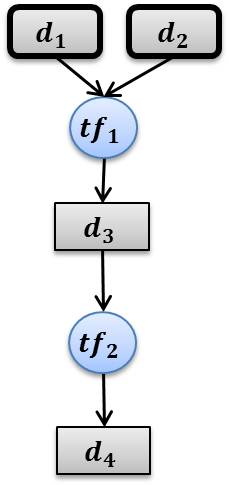
\includegraphics[width=.4\linewidth]{figure/app_model.jpg}
    	\caption{Modelo da aplicação.}
    	\label{app_model}
    \end{subfigure}
    \begin{subfigure}{.5\textwidth}
      \centering
    	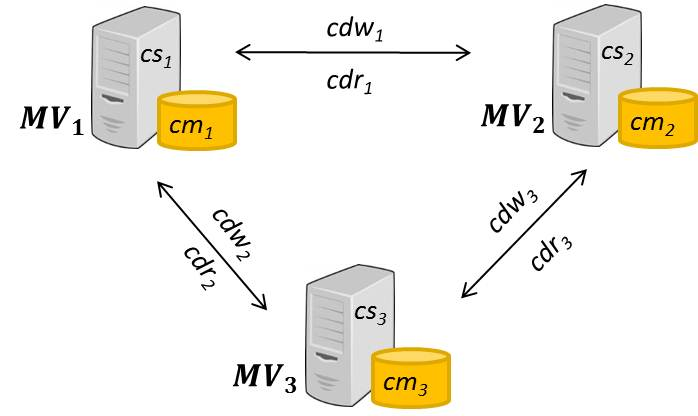
\includegraphics[width=\linewidth]{figure/arch_model1.jpg}
    	\caption{Modelo do Ambiente.}
    	\label{arch_model}
    \end{subfigure}
    \caption{Exemplo dos modelos de ambiente e aplicação.}
    \label{fig:definition}
    \end{figure}

O modelo do ambiente, apresentado na Figura \ref{arch_model}, representa os recursos utilizados durante a execução das aplicações. Nessa representação, o conjunto de todas as MVs disponíveis para execução e armazenamento é dado por $M$. Cada MV $j \in M$ tem capacidade de armazenamento $cm_j$ e um valor computacional de \textit{slowdown} definido como $cs_j$. O \textit{slowdown} representa o grau de diferença da capacidade de processamento das diferentes MVs disponíveis, e é uma alternativa à representação do tempo de execução das tarefas por meio de matrizes \cite{nascimento}. Neste trabalho, o valor de \textit{slowdown} é inversamente proporcional à capacidade de processamento $cp_j$ de uma MV $j$. Porém, nos testes teóricos realizados com \textit{workflows} sintéticos disponíveis na literatura, o valor foi definido em termos dos tempos de execução das tarefas. Essa diferença é explicada no Capítulo \ref{chap6}.



% The architectural model specifies the main features of the target architecture. In order to better reproduce the reality of a large-scale system, let $M$ be the set of all VMs available for execution or storage. Each VM $j \in M$ has a storage capacity $cm_j$ and computational slowdown index $cs_j$, which is inversely proportional to the computational power $cp_j$ of VM $j$, according to Silva \textit{et al.} \cite{nascimento}. 

Seguindo a mesma ideia do \textit{slowdown}, $cd_{l}$  representa o custo de latência associado ao enlace $l$. Dois tipos de retardo de comunicação são propostos: um para a operação de escrita, $cdw_{l}$, e outro para a de leitura, $cdr_{l}$. Por conta disso, duas matrizes de comunicação são construídas, cada uma relacionada a uma das operações de comunicação.  Dessa forma, o tempo de execução da tarefa $i \in N$ na MV $j \in M$ é dado por $t_{ij} = a_i \times cs_j$. Já o tempo de comunicação da tarefa $i \in N$ executando na MV $j \in M$, para escrever e dado $d \in D$ na MV $p \in M$, sendo $j$ e $p$ conectados por um enlace $l$, é dado por $\overleftarrow{t}_{djp} = \omega_{id} \times cdw_{l}$. De modo similar, o tempo de comunicação para leitura é dado por $\overrightarrow{t}_{djp} =  \omega_{di} \times cdr_{l}$. A Figura \ref{arch_model} ilustra um ambiente composto por 3 MVs, contendo as seguintes informações: (i) capacidade de armazenamento $cm$, (ii) valor computacional de \textit{slowdown} $cs$, (iii) o custo de comunicação para operação de escrita ($cdw$) e (iv) o o custo de comunicação para operações de leitura ($cdr$).

A fim de simplificar o modelo, neste trabalho assume-se que um arquivo lido por uma tarefa será mantido na memória principal (volátil). Assim, a operação de leitura não necessita de espaço de armazenamento e não mantém cópia dos dados em diferentes máquinas. 


% 	Moreover, a communication delay index $cd_{l}$ estimates the latency cost associated with each link $l$ of the system. We propose two types of communication delay here. One for the writing cases, $cdw_{l}$, and one for the reading cases, $cdr_{l}$. For supporting our model, two communication delay matrices are built, each one concerning one type of delay. 
%     Therefore, the execution time of a task $i \in N$ on a VM $j \in M$ is given by $t_{ij} = a_i \times cs_j$. 
%     %Let $k \in A$ be an arc connecting task $i \in N$ and data $d \in D$.
%     Furthermore, the communication time for a task $i \in N$ executing on VM $j \in M$, to write data $d \in D$ in VM $p \in M$,  where $j$ and $p$ are connected by link  $l$, is  given by $\overleftarrow{t}_{djp} = \omega_{id} \times cdw_{l}$. Similarly, the communication time for  reading is given by $\overrightarrow{t}_{djp} =  \omega_{di} \times cdr_{l}$. Figure \ref{arch_model} illustrates an example of the architectural model containing three VMs and its characteristics: (i) the storage capacity $cm$, (ii) the computational slowdown index $cs$, (iii) the communication delay index for write operations ($cdw$) and (iv) the communication delay index for read operations ($cdr$).
    
%     Note that when a data is read by some VM, we assume that it is held in main (volatile) memory. Thus, read operations does not require available storage capacity to store data. As future work we intend to tackle the data replication problem in our model. In this way, read operations can take advantage of the nearest replica. 

\subsection{Formulação Matemática}\label{math_form}

O ETAA pode ser formulado como um problema de programação inteira mista, nomeado IP-ETAA, como descrito a seguir. Primeiro, é necessário definir duas classes distintas de arquivos: os arquivos estáticos; e os arquivos dinâmicos. Os arquivos estáticos são aqueles que não são produzidos durante a execução do \textit{workflow} e servem principalmente como entrada para as primeiras tarefas executadas (embora também possam ser utilizados pelas demais tarefas). Um arquivo estático é armazenado antes da execução do \textit{workflow}, em uma das MVs cujo espaço de armazenamento seja suficiente. As alocações desses arquivos não são alteradas em nenhum momento da execução.

Já os arquivos dinâmicos são gerados pelas tarefas como resultado dos processamentos realizados durante a execução do \textit{workflow}. Os arquivos dinâmicos podem ser armazenados em qualquer MV disponível, desde que haja espaço de armazenamento suficiente. A alocação de arquivos, definida como parte do problema deste trabalho, tem a classe de arquivo dinâmicos como foco e, portanto, é papel do escalonador definir a localização desses arquivos.

Sendo assim, $D = D_s \cup D_d$ é definido como sendo o conjunto de todos os arquivos, onde cada arquivo $d \in D$ tem tamanho $W(d)$ e pode ser estático $d \in D_s$ com uma máquina de origem $O(d) \in M$, ou dinâmico $d \in D_d$. Além disso, para cada tarefa $i \in N$ são associados um conjunto de arquivos de entrada $\Delta_{in}(i) \subseteq D$ necessário para sua execução, e um conjunto de arquivos de saída $\Delta_{out}(i) \subseteq D_d$.  Por fim, um tempo $T_M$ é definido como o tempo máximo de execução do \textit{workflow}, sendo $T=\{1 \ldots T_M\}$ o conjunto de intervalos de tempo de uma execução. 

    % The TaSDAP can be formulated as the mixed integer programming problem, named TaSDAP-IP, as described following.
    % Let redefine $D=D_s\cup D_d$ as the set of all data, where each data $d \in D$ has a size $W(d)$ and can be either static ($D_s$), with an origin machine $O(d) \in M$, or dynamic, generated during the workflow execution, ($D_d$). For each $i \in N$,  we consider a set of input data $\Delta_{in}(i) \subseteq D$ needed for it execution and a set of output data 	$\Delta_{out}(i) \subseteq D_d$ generated by it.
    % Moreover, we define $T_M$ as the maximum execution time for the workflow and $T=\{1 ... T_M\}$ as the set of feasible periods.

 
    
    % In this vein, the TaSDAP is defined as the problem of scheduling tasks and assigning data on VMs, respecting the available storage capacity and trying to minimize the makespan. Next, we summarize the data and variables used in the proposed mathematical formulation and present the TaSDAP-IP.
    
    
\begin{table}[h]
\label{tab:desc}\caption{Descrição dos dados e das variáveis utilizadas no modelo matemático.}
\begin{tabularx}{\textwidth}{|l|X|}
\hline
\textbf{Dados}      & \textbf{Descrição}\\
\hline \hline
	$D_s$           &  Conjunto de arquivos estáticos.\\
	$D_d$           &  Conjunto de arquivos dinâmicos.\\
    $D=D_s\cup D_d$ &  Conjunto de arquivos.\\
    $O(d)$          &  Máquina de origem do arquivo estático $d \in D_s$.\\
    $W(d)$          &  Tamanho do arquivo $d \in D$.\\
    $N$             &  Conjunto de tarefas.\\
    $a_i$           &  Quantidade de trabalho da tarefa $i \in N$.\\
    $M$             &  Conjunto de Mvs.\\
    $t_{ij}$        &  Tempo de processamento da tarefa $i \in N$ na Mv $j \in M$. \\
    $\overrightarrow{t}_{djp}$ & Tempo gasto pela Mv $j \in M$ para ler o arquivo $d \in D$ armazenado na Mv $p \in M$\\
    $\overleftarrow{t}_{djp}$  & Tempo gasto pela Mv $j \in M$ para escrever o arquivo $d \in D_d$ na Mv $p \in M$.\\
    $\Delta_{in}(i) \subseteq D$ & Conjunto de arquivos de entrada necessários para a execução da tarefa $i \in N$.\\
    $\Delta_{out}(i) \subseteq D_d$ & Conjnto de arquivos de saída gerados pela tarefa $i \in N$.\\
    $cm_j$          & Capacidade de armazenamento da Mv $j \in M$.\\
    \hline 
    \hline
\textbf{Variáveis}  & \textbf{Descrição}\\
\hline
\hline
    $x_{ijt}$                    & Variável binária que indica se a tarefa $i \in N $ iniciou sua execução na Mv $j \in M$ no período $t \in T$ ou não.\\
    $\overrightarrow{x}_{idjpt}$ & Variável binária que indica se a tarefa $i \in N $ executando na Mv $j \in M$ começou a ler o arquivo  $d \in \Delta_{in}(i)$, que está armazenado na Mv $p \in M$, no período  $t \in T$ ou não.\\
    $\overleftarrow{x}_{djpt}$   & Variável binária que indica se o arquivo $d \in D_d$ começou a ser escrito a partir da Mv $j \in M$ para a Mv $p \in M$ no periodo $t \in T$ ou não.\\
    $y_{djt}$                    & Variável binária que indica se o arquivo $d \in D$ está armazenado na Mv $j \in M$ no período $t \in T$ ou não.\\
    $z_T$                        & Variável contínua que indica o tempo total de execução (\textit{makespan}) do \textit{workflow}.\\
\hline
\end{tabularx}
\end{table}

Como o objetivo do escalonamento é minimizar o tempo total de execução da aplicação, a função objetivo, definida em (\ref{fo}),  minimiza o \textit{makespan} ($z_T$) da aplicação.
% Objetivo
\begin{align}
&\min{z_T} \label{fo}
\end{align}


A restrição (\ref{r1}) garante que cada tarefa seja executada. As restrições (\ref{r2}) e (\ref{r3}) certificam que todas as operações de leitura e escrita sejam realizadas, respectivamente. Já a inequação (\ref{r1}) garante que o dado $d \in \Delta_{out}(i)$ seja escrito apenas se a tarefa $i$ tenha sido executada no tempo correto. Além disso, as restrições definidas em (\ref{r4_1}) asseguram que o dado $d$ não possa ser escrito antes do tempo de processamento da tarefa $i$ (responsável pela sua escrita). Note que ambas as restrições (\ref{r4} e \ref{r4_1}) trabalham em conjunto para garantir um tempo de escrita factível.

% restrições
\begin{align}
&\mathrm{Sujeito\ a\ }  &\nonumber\\
& \sum_{j \in M}\sum_{t \in T} x_{ijt}=1 , & \forall i \in N \label{r1}
\end{align}

\begin{align}
& \sum_{j,p \in M}\sum_{t \in T} \overrightarrow{x}_{idjpt}=1 , & \forall i \in N, \forall d \in \Delta_{in}(i) \label{r2}
\end{align}

\begin{align}
& \sum_{j,p \in M}\sum_{t \in T} \overleftarrow{x}_{djpt}=1 , & \forall d \in D_d \label{r3}
\end{align}

\begin{align}
& \overleftarrow{x}_{djpt} \leq x_{ij(t-t_{ij})} , & \forall d \in D_d, \forall j,p \in M, \nonumber \\ 
&& \forall t = (t_{ij}+1) \cdots T_M  \mbox{ tal que } d \in \Delta_{out}(i)\label{r4}
\end{align}

\begin{align}
& \overleftarrow{x}_{djpt}=0 & \forall d \in D_d, \forall j,p \in M , \nonumber \\ 
&&  1 \leq t \leq t_{ij} \mbox{ tal que } d \in \Delta_{out}(i) \label{r4_1}
\end{align}

A restrição definida em (\ref{r5}) assegura que uma tarefa só possa ser executada quando todas as operações de leitura estiverem concluídas. Além disso, a desigualdade (\ref{r7}) garante que apenas uma ação (execução, leitura ou escrita) possa ser realizada em cada período de tempo em cada MV. Ou seja, a MV não pode executar uma tarefa e escrever, ou ler, um dado ao mesmo tempo.




\begin{align}
& x_{ijt} \leq \sum_{p \in M} \overrightarrow{x}_{idjp(t-\overrightarrow{t}_{djp})} , &\forall i \in N, \forall d \in \Delta_{in}(i), \forall j \in M,\nonumber\\
&& \forall t \in T, \mbox{ tal que }  (t-\overrightarrow{t}_{djp})\geq 1 \label{r5}
\end{align}

\begin{align}
& \sum_{i \in N} \sum_{q=\max{(1,t-t_{ij}+1)}}^t x_{ijq} +  \sum_{d \in D_d} \sum_{p \in M} \sum_{r=\max{(1,t-  \overleftarrow{t}_{djp}+1)}}^t \overleftarrow{x}_{djpr} + &   \nonumber\\
& \sum_{i \in N} \sum_{d \in \Delta_{in}(i)} \sum_{p \in M} \sum_{r=\max{(1,t-  \overrightarrow{t}_{djp}+1)}}^t \overrightarrow{x}_{idjpr} \leq 1 , & \forall j \in M, \forall t \in T  \label{r7}
\end{align}


A restrição (\ref{r8}) estabelece que não há arquivos dinâmicos no tempo inicial. Por outro lado, a restrição (\ref{r9}) garante que todos os arquivos estáticos estejam prontamente armazenados em suas máquinas de origem. Já as restrições (\ref{r10}) e (\ref{r11}) relacionam a variável de armazenamento $y$ com as variáveis de escrita $\overleftarrow{x}$ e de leitura $\overrightarrow{x}$, garantindo um processo viável de escrita e leitura. A restrição (\ref{r11}) garante que os arquivos serão lidos apenas se estes estiverem previamente armazenados em uma MV, e a restrição (\ref{r10}) assegura que um arquivo seja armazenado em MV apenas caso ele tenha sido produzido (escrito).



\begin{align}
& y_{dj1} =0, & \forall d \in D_d, \forall j \in M \label{r8}
\end{align}

\begin{align}
& y_{djt} =1, & \forall d \in D_s \mid j \in O(d), \forall t \in T \label{r9}
\end{align}

\begin{align}
& y_{dp(t+1)} \leq y_{dpt} + \sum_{j \in M} \overleftarrow{x}_{djp(t-\overleftarrow{t}_{djp})} &, \forall d \in D, \forall p \in M, \nonumber\\
&&\forall t \in T, \mbox{ tal que } (t-\overrightarrow{t}_{djp}) \geq 1 \label{r10} 
\end{align}



A capacidade de armazenamento das MVs é estabelecida pela restrição (\ref{r12}). A restrição (\ref{r13}) relaciona a última operação de escrita com o tempo total de execução da aplicação (\textit{makespan}). Note que no modelo da aplicação, uma tarefa sempre escreve ao menos um arquivo. Além disso, a restrição operacional (\ref{r15}) deve ser satisfeita: uma tarefa $i$ pode iniciar um processo de leitura se todos os arquivos $d \in \Delta_{in}(i)$ estiverem disponíveis (isto é, se todos os arquivos $d \in (\Delta_{in}(i) \cap D_d)$ forem escritos). Por fim, as restrições restantes são as de integralidade e de não negativação.



\begin{align}
& \sum_{j \in M} \overrightarrow{x}_{idjpt} \leq y_{dpt} &, \forall i \in N, \forall d \in \Delta_{in}(i), \forall p \in M, \forall t \in T \label{r11}
\end{align}

\begin{align}
& \sum_{d \in D} y_{djt} W(d) \leq cm_j & , \forall j \in M, \forall t \in T \label{r12}
\end{align}

\begin{align}
& \overleftarrow{x}_{djpt}\cdot (t+\overleftarrow{t}_{djp}) \leq z_T & , \forall d \in D_d , \forall j,p \in M, \forall t \in T \label{r13}
\end{align}

\begin{align}
& \overrightarrow{x}_{idjpt} \cdot |\Delta_{in}(i) \cap D_d| \le \sum_{g \in \{\Delta_{in}(i) \cap D_d\}}\sum_{l,o \in M} \sum_{u=1}^{t-\overleftarrow{t}_{glo}}\overleftarrow{x}_{glou} & , \forall i \in N, \forall d \in \Delta_{in}(i), \nonumber \\
&&\forall j,p \in M, \forall t \in T \label{r15}
\end{align}







    % The objective function (\ref{fo}) minimizes the application makespan. 
    % %
    % Constraints (\ref{r1}) guarantee that every task must be executed. Constraints (\ref{r2}) and (\ref{r3}) rule that every read and write operations must be accomplished, respectively. 
    % % %
    % Inequalities (\ref{r4}) guarantee that data $d \in \Delta_{out}(i)$ can only be written, if task $i$ was executed in the correct time. Furthermore, constraints (\ref{r4_1}) rule that data $d$ can not be written before the processing time of the task $i$ (responsible for its writing). Note that both sets of constraints ((\ref{r4}) and (\ref{r4_1})) work together to guarantee a feasibly time for the writing process.
    %
    % Constraints (\ref{r5}) rule that a task can only be executed, if all necessary readings were concluded in a feasible time.
    % %
    % Inequalities (\ref{r7}) guarantee that only one action (execution, reading or writing) can be accomplished at each period of time in each VM (e.g. a VM cannot execute a task and write data at the same time). 
    % %
    % Constraints (\ref{r8}) establish that there are no dynamic data at starting time. On the other hand, constraints (\ref{r9}) guarantee that all static data are already stored on its origin machines. 
    % %
    % % Constraints (\ref{r10}) and (\ref{r11}) link the storage variable $y$ with the write variable $\overleftarrow{x}$ and the read variable $\overrightarrow{x}$, guaranteeing a feasible write and read process, respectively.
    % %
    % In detail, constraint (\ref{r11}) ensures that data will only be read if previously stored in a VM, and constraint (\ref{r10}) ensures that data will only be stored in a VM, if it has been already produced (written). 
    
    % The VMs storage capacity are bounded by constraints (\ref{r12}).
    % %
    % Constraints (\ref{r13}) relate the last write operation with the application execution time (makespan). Note that in our application model a task always creates data.
    % %
    % Moreover, the following operational constraint (\ref{r15}) must be satisfied: a task $i$ can only begin any reading process if all data $d \in \Delta_{in}(i)$ is already available (\textit{i.e.}, if all data $d \in (\Delta_{in}(i) \cap D_d)$ is written).
    % %Constraints (\ref{r14}) make sure that a data replication occurs from a machine that has the content.
    % %
    % Finally, the remaining constraints are the integrality and non-negativity constraints.
%